\section{Introduction}

\label{sec:sec1}

In 1950s, a series of experiments performed by R.~Hofstadter~\cite{Hofstadter:1956qs} revealed that nucleons have a substructure 
(which corresponds to our modern view in terms of quarks and gluons).
The experiment confirmed M.~Rosenbluth's theory of electron scattering~\cite{Rosenbluth:1950yq} based on the one-photon exchange approximation.
In this so-called Born approximation, where the interaction between the electron and the nucleon occurs $via$ an exchange of one virtual photon (OPE), 
the unpolarized $e-N$ elastic cross section can be parameterized in terms of a nucleon magnetic, \gmf, and electric, $G_E$, form factors. 
These form factors describe the deviation from a point-like scattering cross section, $\sigma_{_{Mott}}$:  

\begin{equation}\label{eq:Ros}
\bigg(\frac{d\sigma}{ d\Omega}\bigg)_{eN\rightarrow eN}  = \frac{\sigma_{_{Mott}}}{\epsilon(1+\tau)}\;\; 
\big[ \tau \cdot G^{2}_{_M}(Q^2) + \epsilon \cdot G^{2}_{_E}(Q^2)\big] ,
\end{equation}
\vskip .25 in
 where $E$ and $E'$ are the incident and scattered electron energies, respectively, $\theta$ is the electron scattering angle, 
$\tau \equiv -q^{2}/4M^{2}$,  with $-q^2 \equiv Q^2 = 4EE'\sin{(\theta/2)}$ being the negative four momentum transfer squared, 
$M$ is the nucleon mass, and $\epsilon = \big[ 1 + 2(1+\tau) \tan^2{(\theta/2)} \big]^{-1}$ is the longitudinal polarization 
of the virtual photon. The reduced cross section is defined by:
\begin{equation}\label{eq:reduced}
\sigma_r \equiv \bigg(\frac{d\sigma}{ d\Omega}\bigg) \cdot \frac{\epsilon(1+\tau)}{\sigma_{_{Mott}}}\;\; 
= \tau \cdot G^{2}_{_M}(Q^2) + \epsilon \cdot G^{2}_{_E}(Q^2) \;=\; \sigma_{_T} + \epsilon \cdot \sigma_{_L},
\end{equation}
\vskip .25 in

where $\sigma_{_L}$ and $\sigma_{_T}$ are the cross sections for longitudinally and transversely polarized virtual photons, respectively.

\begin{figure}[!h]
  %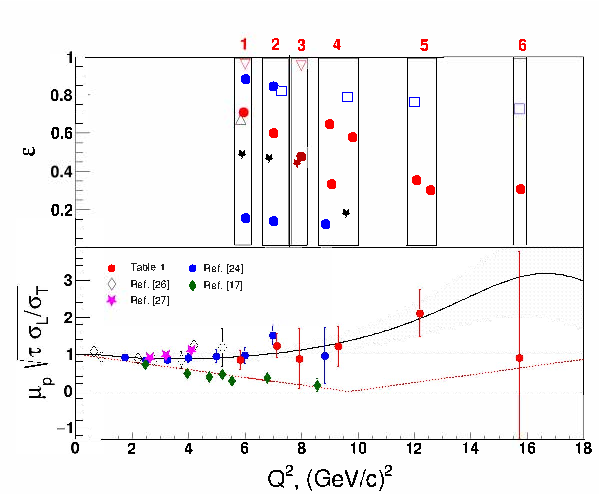
\includegraphics[trim = 0mm 0mm 0mm 40mm, width = 0.75\textwidth]{Plots/Fig1.pdf}
  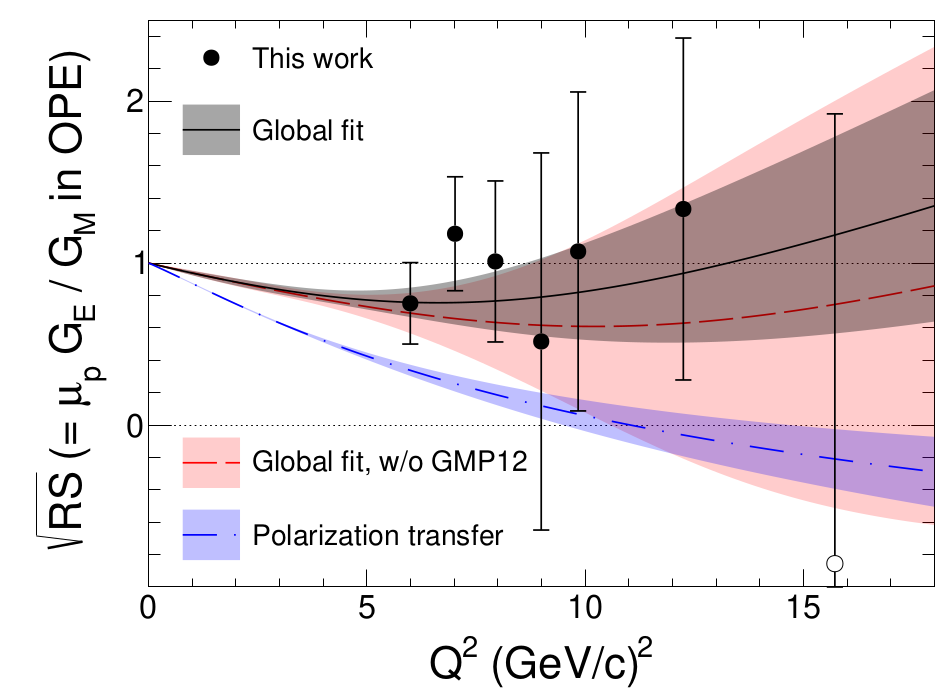
\includegraphics[width = 0.75\textwidth]{Plots/Fig1-final.png}
\caption{The square root of Rosenbluth slope, corrected for kinematical factor $\sqrt {\tau}$ and $\mu_p$, observed in elastic electron-proton scattering,
adopted from Ref.~\cite{Christy2020ab}. References in the plot are also from Ref.~\cite{Christy2020ab}}
\label{pic:Fig1}
\end{figure}

The linear $\epsilon$ dependence of the cross section is due to the $\sigma_{_L}$ term. %, see Eq.~\ref{eq:Ros}.
The ratio $\sigma_{_L}/\sigma_{_T}$ is the so-called Rosenbluth slope related to \gef/\gmf (in OPE), see Fig.~\ref{pic:Fig1}.
The data show that at \qsq~of 4-5 \gevcsq~the Rosenbluth slope is three to four times larger than expected in OPE (shown as the dot-dashed line in Fig.~\ref{pic:Fig1}) for the observed values of the \gep/\gmp~ratio.

%
The nucleon electromagnetic form factors can reveal a lot of information about the nucleon internal structure, as well as the quark distribution. 
The form factors depend only on one variable, the negative square of the four-momentum transfer carried by the photon, \qsq. 
In the limit of large \qsq, perturbative QCD (pQCD) provides well-motivated predictions for the \qsq-dependence of the form factors and their ratio. 
However, it was never predicted at what \qsq~range the pQCD prediction (scaling) will be valid.
Studies show that pQCD validity will require a very large \qsq~of 100~\gevcsq.
It was discovered at JLab, using the double polarization methods, that the proton electric and magnetic form factors behave differently starting at \qsq~ $\approx$ 1~\gevcsq.
%even below \qsq~ $\approx$ 1~\gevcsq. ?
 
\begin{figure}[!h]
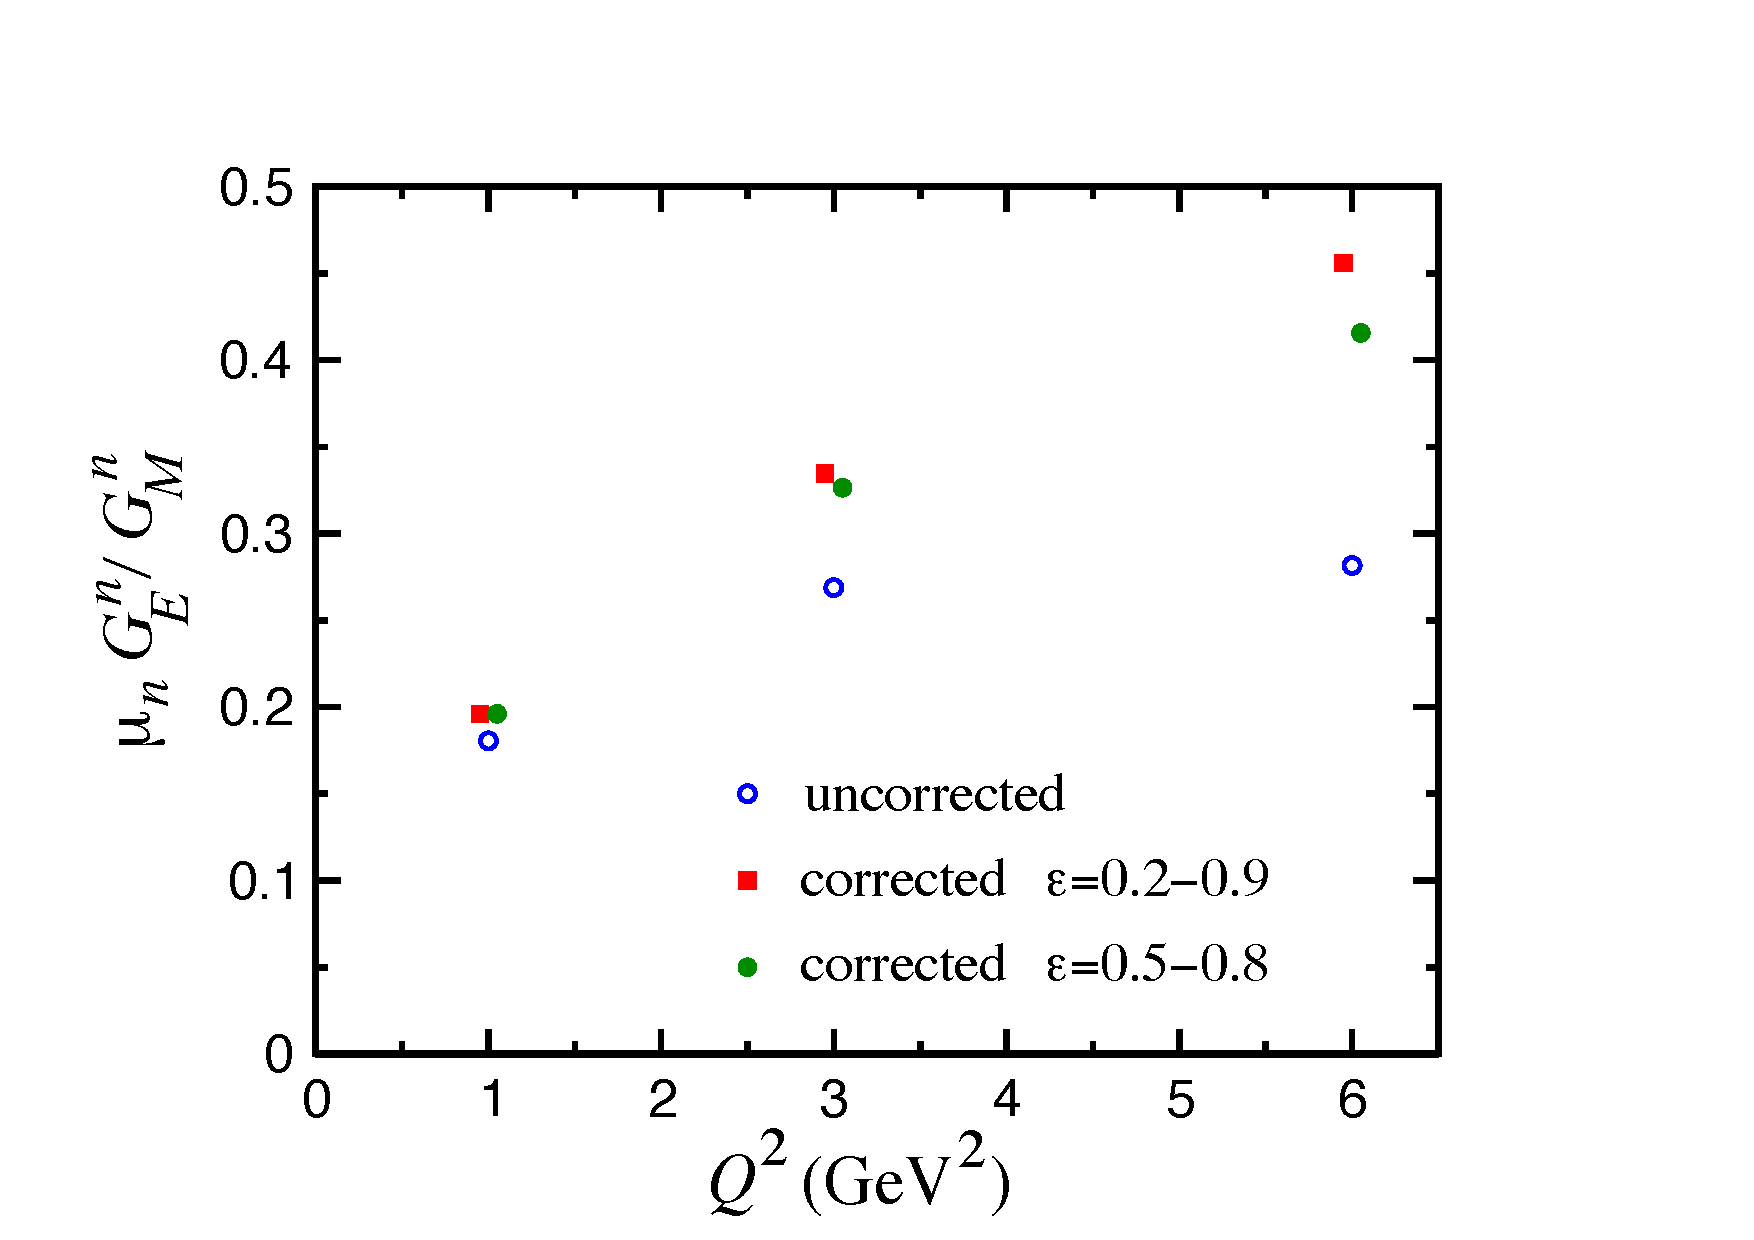
\includegraphics[width = 0.95\textwidth]{Plots/nTPE-BMT.pdf}
\caption{Projected impact of TPE on \gen/\gmn~using LT separation, according to Ref.~\cite{Blunden:2005ew}.}
\label{pic:Fig2}
\end{figure}
 
Experimentally, the nucleon form factors can be measured using one of two techniques: the polarization transfer technique and the Rosenbluth technique. 
The polarization method examines the polarization transfer from longitudinally polarized electron to the recoiling nucleon and 
determine the resulting azimuthal asymmetry distribution using a polarimeter. 
Alternatively, one can use a polarized electron beam and polarized target. 
In the Rosenbluth method, the electric and magnetic from factors can be separated by making two or more measurements with 
different $\epsilon$ values ($i.e.$ different beam energies and angles), but with same \qsq~value. 
The Rosenbluth technique requires an accurate measurement of the cross section and suffers from large systematic uncertainties arising from several factors, for instance
the need for a precise determination of the scattering angle. Additionally,
for a measurement of the neutron form factors, accurate knowledge of
the neutron detector efficiency is required, which is particularly hard to
achieve.
These uncertainties can be greatly reduced by measuring the ratio of $e-n$ and $e-p$ quasi-elastic cross sections.
%large systematic uncertainties arising from several factors. 
%For instance, an accurate knowledge of the neutron detector efficiency is required.

When comparing the values of \gep/\gmp~obtained from both techniques, a significant discrepancy was observed (see Fig.~\ref{pic:Fig1}). 
Such a discrepancy implies a potential problem in our understanding of the nucleon substructure. 
Many efforts were made to explain this effect, and it is believed that the inconsistency is due to the contribution of two-photon exchange
in $e-N$ elastic scattering process~\cite{Arrington:2011dn, Afanasev:2017gsk}.
While the two-photon exchange is currently considered as the most likely explanation for this discrepancy, there is still debate on whether it is the only source.
Fortunately, this contribution is also dependent on the charge of the lepton, meaning that it will contribute differently to the Rosenbluth slope on $e^--N$ and $e^+-N$.

Predictions made for the electron-neutron case are shown in Fig.~\ref{pic:Fig2}, adopted from~\cite{Blunden:2005ew}.
Experiment E12-20-010 (currently under analysis) measured for the first time the Rosenbluth slope in $e^--n$.
that a similar measurement as E12-20-010~\cite{ntpe} on positron neutron scattering is expected to give a different slope.

%The contribution of TPE could reach about 30\% of the Rosenbluth slope value at 5 \gevcsq.
%In the following we propose to make a precision L/T separation of the elastic electron-neutron cross section and first experimental assessment 
%of the two-photon exchange contribution on the neutron magnetic form factor measurements (see also Ref.~\cite{Wojtsekhowski:2017kti}).
%The result of the nTPE experiment will likely add a new component to our understanding of the elastic electron-nucleon process.
